\documentclass[
  digital,     %% The `digital` option enables the default options for the
               %% digital version of a document. Replace with `printed`
               %% to enable the default options for the printed version
               %% of a document.
%%  color,       %% Uncomment these lines (by removing the %% at the
%%               %% beginning) to use color in the printed version of your
%%               %% document
  oneside,     %% The `oneside` option enables one-sided typesetting,
               %% which is preferred if you are only going to submit a
               %% digital version of your thesis. Replace with `twoside`
               %% for double-sided typesetting if you are planning to
               %% also print your thesis. For double-sided typesetting,
               %% use at least 120 g/m² paper to prevent show-through.
  nosansbold,  %% The `nosansbold` option prevents the use of the
               %% sans-serif type face for bold text. Replace with
               %% `sansbold` to use sans-serif type face for bold text.
  nocolorbold, %% The `nocolorbold` option disables the usage of the
               %% blue color for bold text, instead using black. Replace
               %% with `colorbold` to use blue for bold text.
  lof,         %% The `lof` option prints the List of Figures. Replace
               %% with `nolof` to hide the List of Figures.
  lot,         %% The `lot` option prints the List of Tables. Replace
               %% with `nolot` to hide the List of Tables.
]{fithesis4}
%% The following section sets up the locales used in the thesis.
\usepackage[resetfonts]{cmap} %% We need to load the T2A font encoding
\usepackage[
  main=english, %% By using `czech` or `slovak` as the main locale
                %% instead of `english`, you can typeset the thesis
                %% in either Czech or Slovak, respectively.
  % english, german, russian, czech, slovak %% The additional keys allow
]{babel}        %% foreign texts to be typeset as follows:
%%
%%   \begin{otherlanguage}{german}  ... \end{otherlanguage}
%%   \begin{otherlanguage}{russian} ... \end{otherlanguage}
%%   \begin{otherlanguage}{czech}   ... \end{otherlanguage}
%%   \begin{otherlanguage}{slovak}  ... \end{otherlanguage}
%%
%% For non-Latin scripts, it may be necessary to load additional
%% fonts:
\usepackage{paratype}
% \def\textrussian#1{{\usefont{T2A}{PTSerif-TLF}{m}{rm}#1}}
%%
%% The following section sets up the metadata of the thesis.
\thesissetup{
    date        = \the\year/\the\month/\the\day,
    university  = mu,
    faculty     = fi,
    type        = bc,
    department  = Department of Computer Systems and Communications,
    author      = Dominik Tichý,
    gender      = m,
    advisor     = {RNDr. Tomáš Raček, Ph.D.},
    title       = {Modern visualization of partial atomic charges in Mol*},
    TeXtitle    = {Modern visualization of partial atomic charges in Mol*},
    keywords    = {%
        Molstar,
        Mol*,
        Atomic Charge Calculator 2,
        ACC2,
        AlphaCharges,
        αCharges,
        SB NCBR,
        molecular visualization,
        molecular graphics,
        partial atomic charges,
        structural biology,
        AlphaFold
     },
    TeXkeywords = {%
        Molstar,
        Mol*,
        Atomic Charge Calculator 2,
        ACC2,
        AlphaCharges,
        αCharges,
        SB NCBR,
        molecular visualization,
        molecular graphics,
        partial atomic charges,
        structural biology,
        AlphaFold
    },
    abstract    = {%
        TODO
    },
    thanks      = {%
        TODO
    },
    bib         = {%
        main.bib,
    },
    %% Remove the following line to use the JVS 2018 faculty logo.
    facultyLogo = fithesis-fi,
}
\usepackage{tipa}
\usepackage{makeidx}      %% The `makeidx` package contains
\makeindex                %% helper commands for index typesetting.
%% These additional packages are used within the document:
\usepackage{paralist} %% Compact list environments
\usepackage{amsmath}  %% Mathematics
\usepackage{amsthm}
\usepackage{amsfonts}
\usepackage{url}      %% Hyperlinks
\usepackage{markdown} %% Lightweight markup
\usepackage{listings} %% Source code highlighting
\lstset{
  basicstyle      = \ttfamily,
  identifierstyle = \color{black},
  keywordstyle    = \color{blue},
  keywordstyle    = {[2]\color{cyan}},
  keywordstyle    = {[3]\color{olive}},
  stringstyle     = \color{teal},
  commentstyle    = \itshape\color{magenta},
  breaklines      = true,
}
\usepackage{floatrow} %% Putting captions above tables
\floatsetup[table]{capposition=top}
\usepackage[babel]{csquotes} %% Context-sensitive quotation marks
\usepackage{minted}
\usepackage{subfigure}
\usepackage{textalpha}

\begin{document}

\chapter*{Introduction}
\markright{\textsc{Introduction}}
\addcontentsline{toc}{chapter}{Introduction}

\chapter{Theory}
\label{chapter:theory}

\textbf{TODO}: this chapter is has placeholder text and is not finished yet. \\

Theoretical concepts are fundamental to the study of computational chemistry, providing a framework for analyzing molecular structures and properties. This chapter focuses on four key areas of theory, beginning with an overview of molecular structure in Section 1.1. Section 1.2 provides an in-depth examination of chemical file formats, including the advantages and disadvantages of different file formats for storing molecular data. Partial atomic charges are explored in section 1.3, including their importance in analyzing molecular structures and the various methods used to compute them. Finally, section 1.4 delves into color interpolation, a critical technique for visualizing partial atomic charges in molecular structures.

By providing a comprehensive overview of these theoretical concepts, this chapter provides a strong foundation for the subsequent chapters, focusing on the implementation and analysis of the Mol* extension for visualizing partial atomic charges in molecular structures.

\section{Molecular structure}
\label{section:molecular_structure}

\textbf{TODO}: the section is not split into many subsections to allow for better reading flow; first i describe small molecules (micromolecules) which are just described by their atoms and bonds, these are usually drug molecules (think ligands, ions etc); for macromolecules explain the hierarchy of chain-residue-atom, in this work we used carbohydrates and proteins - describe those as well; explain somehow that this separation is done on purpose; add a schematic image that shows a small protein with 2 chains, then zoom in on one chain and show the residues, lastly zoom on one of the residues to show the atoms and bonds \\

\textbf{TODO}: don't focus too much on explaining things that aren't relevant further in the thesis \\

\subsection{Micromolecules}

\subsection{Macromolecules}

Molecular structure refers to the arrangement of atoms and chemical bonds in a molecule. The three main components of molecular structure are atoms, residues, and chains.
In this section we will look at

Atoms are the basic building blocks of matter. Atoms are composed of protons, neutrons, and electrons. The number of protons determines the element, while the number of neutrons determines the isotope. The number of electrons determines the charge of the atom. Atoms are the smallest unit of matter that can take part in a chemical reaction.

Bonds are the connections between atoms that hold molecules together. There are different types of bonds, e.g. covalent bonds, ionic bonds, and hydrogen bonds.

A residue refers to a specific building block that remains after a chemical modification or enzymatic reaction.
In proteins, residues refer to amino acids, which are connected through peptide bonds to form polypeptide chains.
Residues are crucial in biochemistry because they determine the structure and function of biological molecules.
The sequence of residues in a protein or nucleic acid, for instance, determines its three-dimensional structure and ultimately its biological activity.

Polymer chains (chains) are sequences of residues that are linked together. In the context of biomolecules, chains can be either polypeptide chains in proteins or polynucleotide chains in nucleic acids. The sequence and structure of these chains are crucial for understanding the function and properties of the biomolecules.

Alternative conformations, also referred to as conformational isomerism, are different conformations of the same molecule. They can be used to represent different states of a molecule, such as different protonation states or different ligand binding modes. Alternative conformations are important for understanding the structure and function of biomolecules, as they provide insight into how they interact with other molecules.

\begin{figure}[htbp]
  \centering
  \subfigure[Residues of chain B.]{\label{fig:structure1}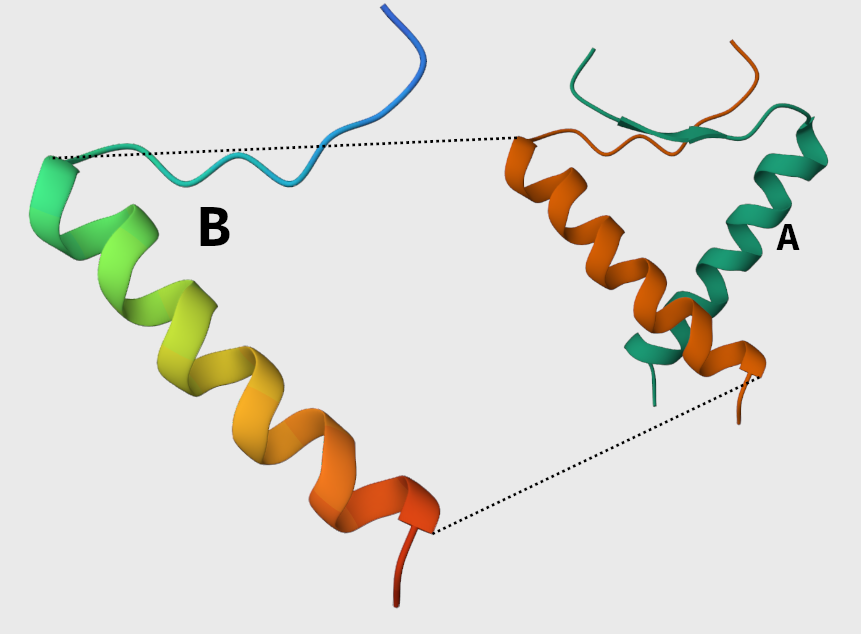
\includegraphics[height=4.5cm]{figures/structure1.png}}
  \subfigure[Atoms of residue ARG 19.]{\label{fig:structure2}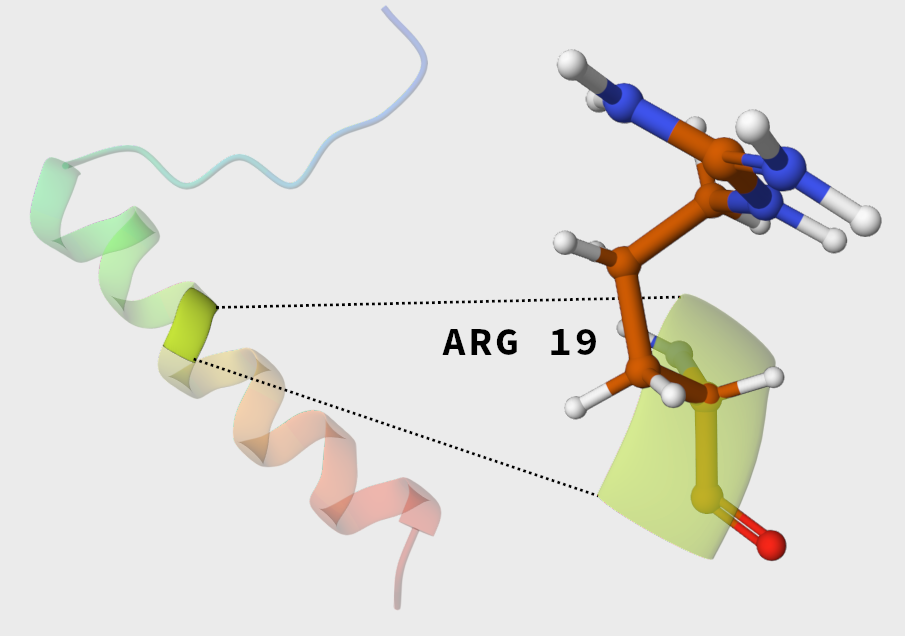
\includegraphics[height=4.5cm,]{figures/structure2.png}}
  \caption{Hierarchy of structure 1A1U.}
  \label{fig:partial_charges_color_theme}
\end{figure}


\section{Partial atomic charges}
\label{section:partial_atomic_charges}

\textbf{TODO}: this section will describe partial atomic charges, their applications, then it will describe how they are calculated using quantum mechanics, explain the need for empirical methods, describe empirical methods, and lastly mention chargefw2 and alphacharges as applications that use the empirical methods \\

Partial atomic charges are numerical values assigned to individual atoms within a molecule, representing their contribution to the overall charge distribution. These charges provide information about the electron density and the distribution of positive and negative charges within the molecule.

There are several applications for partial atomic charges in computational chemistry, including molecular dynamics simulations, molecular docking, and molecular mechanics.

\begin{itemize}
  \item Molecular dynamics - are used to simulate the motion of molecules over time. It is used to study the dynamics of molecules, such as proteins and nucleic acids.
  \item Molecular docking is used to predict the binding affinity of a ligand to its receptor. It is used to study the interactions between molecules, such as proteins and nucleic acids.
  \item Molecular mechanics is used to calculate the energy of a molecule. It is used to study the stability of molecules, such as proteins and nucleic acids.
\end{itemize}

\subsection{Empirical methods}

However, the quantum mechanics of molecules is too complex to be solved analytically. Therefore, empirical methods are used to approximate the electron density and the distribution of positive and negative charges within the molecule.

\section{Chemical file formats}
\label{section:chemical_file_formats}

\textbf{TODO}: this section describes the file formats used during the thesis work; i will briefly describe SDF, MOL2, and PDB focus in more detail on the mmCIF file format: i will explain the data dictionaries; show one example molecule in each file format for SDF-MOL2 and PDB-mmCIF \\

Chemical file formats are used to store molecular data in a computer-readable format. There are many file formats for storing molecular data, each suited to a specific purpose. This section provides an overview of the most common file formats used in computational chemistry.

\subsection{SDF}
\label{subsection:sdf}

Structure-data file (SDF) is a widely used chemical file format for representing molecular structures and their associated properties. It is a text-based format that describes the atoms, bonds, and atomic coordinates of a molecule. 

\subsection{MOL2}
\label{subsection:mol2}

The Mol2 file format is another text-based format for storing molecular structures and their associated properties. It can store multiple conformations of a molecule and is commonly used in molecular modeling and cheminformatics applications. The Mol2 format provides more flexibility and additional features compared to the SDF format, such as support for multiple substructures and atom types.

\subsection{PDB}
\label{subsection:pdb}

\cite{gu2009structural}

The Protein Data Bank (PDB) file format is a widely used format for storing three-dimensional structures of proteins, nucleic acids, and other macromolecules. PDB files contain information about the atomic coordinates, secondary structure, and other important details required for understanding macromolecular structures. The PDB format has been widely adopted in structural biology, bioinformatics, and related fields.

\subsection{mmCIF}
\label{subsection:mmcif}

\textbf{TODO}: explain the need for creating the mmCIF file format, why isn't the PDB format enough (limited amount of rows, poor support for extending the format to add custom data)? describe the mmcif file format; make sure to explain the core data dictionaries, can mention binary cif \\

\cite{gu2009structural}

The macromolecular Crystallographic Information File (mmCIF) format is an extension of the CIF format, specifically designed for macromolecular structures.
It is a text-based format that provides a more comprehensive and flexible representation of macromolecular crystallography data compared to the PDB format.
One of the most important features of the mmCIF format is its support for data dictionaries.
This allows users to define new data items and integrate additional information.
In contrast to other formats, the mmCIF format does not impose limits on column width and entry count, making it more flexible and accommodating for storing large amounts of data.

TODO: add example image + better explanation

\section{Color interpolation}
\label{section:color_interpolation}

\textbf{TODO}: this section will briefly describe color interpolation, add math equation so that it looks pro, add example of interpolations used in the partial charges color theme \\

Color interpolation is the process of creating new colors by mixing two or more colors together. It is a common technique used in computer graphics and digital image processing to create smooth transitions between colors.

Color interpolation works by calculating the intermediate colors between two or more given colors. This is typically done by taking a weighted average of the red, green, and blue values of the colors being interpolated.

TODO: add math equation + image of red,white and white,blue interpolation

\chapter{Visualizing molecular data}
\label{chapter:visualizing_molecular_data}

\section{Types of visualizations}
\label{section:types_of_visualizations}

\textbf{TODO}: thinking about merging the types of visualizations into one section like i did with the molecular structure \\

There are several methods to represent molecular data, each serving a different purpose and providing a different level of detail. The methods most relevant to this work are the following three types: ball and stick, surface, and cartoon.

\subsection{Ball and stick}
\label{subsection:ball_and_stick}

The ball and stick model represents atoms as spheres and bonds as cylindrical connections between these spheres. This model provides a simple and intuitive visualization of a molecule's atomic structure. It highlights individual atoms and their bonds, including their bond types. However, it may not accurately represent the spatial relationships between atoms in larger molecules or macromolecular complexes.

An example of a ball and stick model is shown in Figure \ref{fig:partial_charges_color_theme-bas}.

\subsection{Surface}
\label{subsection:surface}

Surface representations depict the three-dimensional shape of a molecule by displaying its solvent-accessible surface.
This model provides a more accurate representation of the molecule's overall shape and size, making it especially useful for studying macromolecular interactions and the binding of small molecules.
For example, surface visualization can be used to identify potential binding sites on a protein surface, which can then be targeted by drug molecules.

An example of a surface model is shown in Figure \ref{fig:partial_charges_color_theme-surface}.

\subsection{Cartoon}
\label{subsection:cartoon}

Cartoon representations simplify the molecular structure by focusing on the secondary structure elements of proteins and nucleic acids, such as alpha helices, beta sheets, and loops. Alpha helices are often depicted as a spiral-like structures, whereas beta sheets as arrows. This type of visualization is particularly useful for visualizing large macromolecular complexes, as it highlights the overall organization and topology of the molecule without the clutter of atomic details. The simplification of the structure also makes it easier to understand the folding and dynamics of the molecule.

An example of a cartoon model is shown in Figure \ref{fig:partial_charges_color_theme-cartoon}.

\section{Coloring of molecular visualizations}
\label{subsection:coloring_of_molecular_visualizations}

\textbf{TODO}: select a handful of color themes; don't list them out; instead describe them in text and give examples of how they are used by researchers \\

Equally important as the type of visualization is the coloring scheme used to represent the molecule. Coloring is an essential aspect of molecular visualization, as it can provide additional information and help to emphasize specific features or properties of the molecule. Some common coloring schemes include:

\begin{itemize}
  \item \textbf{Element symbol}: atoms are colored according to their chemical element (e.g., carbon in grey, oxygen in red, nitrogen in blue).
  \item \textbf{Partial charge}: atoms are colored according to their partial charge (e.g., positive in blue, negative in red).
  \item \textbf{B-factor}: atoms are colored according to their B-factor value (e.g., low in blue, high in red).
  \item \textbf{Residue index}: atoms or residues are colored according to their residue index (e.g., low in blue, high in red).
  \item \textbf{Residue type}: atoms or residues are colored according to their residue type (e.g., hydrophobic in green, hydrophilic in blue).
  \item \textbf{Chain identifier}: atoms or residues are colored according to their chain identifier (e.g., chain A in blue, chain B in red).
  \item \textbf{Atom type}: atoms are colored according to their atom type (e.g., carbon in grey, oxygen in red, nitrogen in blue).
  \item \textbf{Secondary structure}: Residues are colored according to their secondary structure type (e.g., alpha helix in red, beta sheet in blue).
  \item \textbf{Hydrophobicity}: atoms or residues are colored according to their hydrophobicity. Hydrophobic residues are depicted in green, hydrophilic residues in blue.
\end{itemize}


\section{Visualization software}
\label{section:visualization_software}

\textbf{TODO}: describe the web based \\

There are numerous software tools available for visualizing molecular data, with varying levels of complexity, customization, and features. Some of the most popular tools include MolScript \cite{kraulis1991molscript}, PyMOL \cite{delano2002pymol}, VMD \cite{humphrey1996vmd}, and ChimeraX \cite{goddard2018ucsf}. More recently, web-based tools, such as NGL Viewer \cite{rose2015ngl}, LiteMol \cite{sehnal2017litemol}, and Mol* \cite{sehnal2021molstar}, have become increasingly popular due to their accessibility and ease of use. Furthermore, these web-based tools are especially useful for visualizing large macromolecular complexes, which are becoming increasingly common due to advances in structural biology techniques such as crystallography and electron microscopy. \cite{sehnal2021molstar}

In the following sections, we will discuss the two web-based molecular visualization tools used in this work: LiteMol and Mol*.

\subsection{Litemol}
\label{subsection:litemol}

LiteMol is an open-source, web-native molecular visualization tool that supports various file formats and offers a user-friendly interface for creating visualizations. LiteMol provides essential visualization types, including ball and stick, surface, and cartoon representations, as well as options for customizing colors, lighting, and other display settings. The web-based nature of LiteMol makes it easily accessible and platform-independent.

The LiteMol suite is a freely available tool for visualizing large macromolecular structure datasets, which consists of three components: data delivery services, a compression format, and a lightweight 3D molecular viewer. It enables fast delivery and visualization of large datasets and is compatible with modern web browsers and mobile devices, making it accessible to users with and without structural biology expertise. The tool addresses the challenges of delivering and visualizing large structural data sets, which are becoming increasingly available due to advances in electron microscopy and other techniques. \cite{sehnal2017litemol}

\subsection{Mol*}
\label{subsection:molstar}

Mol* (/'molstar/) is another web-native molecular visualization tool, developed as part of the wwPDB OneDep system for macromolecular structure deposition and validation. Mol* offers a wide range of visualization options, including advanced features such as electron density maps and validation reports. Mol* supports many file formats, including PDB, mmCIF, and PDBx/mmJSON. Like LiteMol, Mol* is platform-independent and can be accessed from any web browser. \cite{sehnal2021molstar}

Mol* emphasizes interactivity and offers various tools for manipulating and analyzing the molecular structure, such as distance and angle measurements, selection and display of specific residues, and custom coloring schemes. Additionally, Mol* provides integration with external databases and services, such as UniProt, PDBe, and RCSB PDB, enabling users to quickly access related information and resources.

\chapter{Mol* partial charges extension}
\label{chapter:molstar_partial_charges_extension}

Visualizing partial atomic charges in molecules is an essential aspect of computational chemistry research, aiding in analyzing complex molecular structures. Mol* provides an extensive range of features for users to explore molecular structures. However, the tool lacks the functionality to color and label atoms and residues based on their partial atomic charges.
This can be a considerable limitation for researchers. In response to this need, we have created an extension to Mol* that addresses this limitation.

It should be noted that the Mol* viewer predecessor, Litemol, supported this functionality. However, since Litemol is no longer supported, we saw the need to bring this functionality to Mol*.

This chapter describes the requirements for the extension, the custom mmCIF categories necessary for storing the partial atomic charges, and the implementation of the extension itself.

\section{Requirements}
\label{section:requirements}

TODO: describe what residue charges are \\
TODO: describe what each representation should visualize when colored using partial charges coloring \\

Firstly, the extension should enable the coloring of atoms and residues based on their partial atomic charges. Secondly, it should describe the charge values of the atoms and residues. Thirdly, the extension should allow the user to provide multiple charge sets for a single structure and select which one to display. Finally, the extension should be seamlessly integrated into the Mol* library, facilitating access to its features and functionality.

\section{Mol* state tree}

After loading a structure the Mol* viewer loads the structure into a state tree. The state tree is a tree structure that contains node which can be anything really. At the leaves of the tree are 3D Representations of the parent selections. The selections are just a collection of atoms that should be visualized.

\begin{figure}
  \begin{center}
    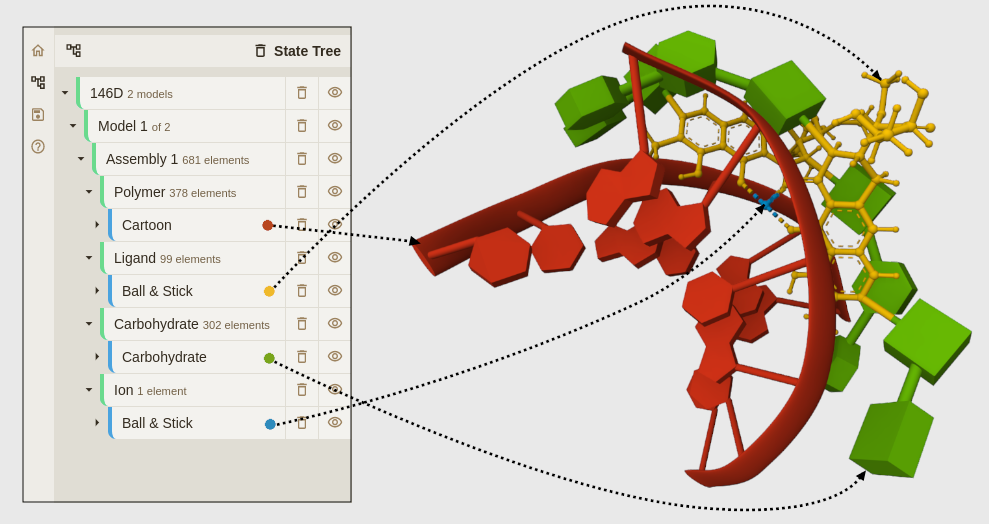
\includegraphics[width=\textwidth]{figures/state_tree.png}
  \end{center}
  \caption{Mol* state tree.}
  \label{fig:state_tree}
\end{figure}

\section{Custom mmCIF categories}
\label{section:custom_mmcif_categories}

To store partial atomic charges within a single file, we developed custom categories within the mmCIF format. The mmCIF format was chosen because it is widely used in the field of structural biology and offers several advantages over other formats, as discussed in \ref{subsection:mmcif}. The custom categories allow us to store information about the partial atomic charges separately from the other structural data, while still being able to access it within the same file. Storing all data in one file was important as it allowed for easier management and distribution of the data. If the charges were stored separately, we would have to provide the charge data to Mol* in a different way e.g. through custom import controls.


We used two separate categories for this purpose: one to store the partial charge values for each atom in the structure, and another to store metadata about the charge sets.

The category \texttt{\_sb\_ncbr\_partial\_atomic\_charges} maps together the atoms of the structure and their charges. The category has three attributes:

\begin{itemize}
  \item \texttt{type\_id} - pointer to the \\ \texttt{\_sb\_ncbr\_partial\_atomic\_charges\_meta.id} item
  \item \texttt{atom\_id} - pointer to the \texttt{\_atom\_site.id} item described in \ref{subsection:mmcif}
  \item \texttt{charge} - partial charge value for the atom
\end{itemize}

The category \texttt{\_sb\_ncbr\_partial\_atomic\_charges\_meta} is dedicated to storing metadata about the charge sets. The metadata category has the following attributes:

\begin{itemize}
  \item \texttt{id} - unique identifier for the charge set
  \item \texttt{type} - type of the calculation method (e.g. 'empirical', 'quantum')
  \item \texttt{method} - computation method used to calculate the charge set (e.g. 'EQeq', 'EEM/Racek 2016 (ccd2016\_npa)')
\end{itemize}

Figure \ref{fig:mmcif_erd} provides a detailed illustration of the custom mmCIF categories and their relationships.

\begin{figure}
  \begin{center}
    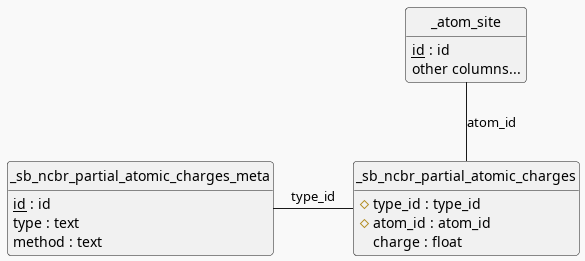
\includegraphics[width=\textwidth]{figures/mmcif_erd.png}
  \end{center}
  \caption{Diagram of custom mmCIF categories.}
  \label{fig:mmcif_erd}
\end{figure}

\section{Implementation}
\label{section:implementation}

This section will detail the implementation of the extension. The extension consists of multiple providers. Each provider serves a distinct functionality, such as supplying the partial charge data and coloring the structural elements based on their charges. The providers will be described in detail in the following subsections.

The extension was created using TypeScript, a superset of JavaScript that adds static typing and other features to the language. The Mol* library is also written in TypeScript, so the extension was written in the same language to ensure compatibility.

\subsection{Property provider}
\label{subsection:property_provider}

In order to retrieve the charges from the mmCIF file, it is necessary to parse the file. This is done by the Mol* library, which parses the mmCIF file and provides the parsed mmCIF file data in the form of a \texttt{MmcifFormat} object. The purpose of this provider is to process the charge data from this object and supply the charge data to the rest of the extension providers through a custom property. The interface of this property is depicted in Figure \ref{figure:charge_data_structure}.

The atom charges are stored in the \texttt{typeIdToAtomIdToCharge} map. The map is indexed by the charge set (typeId) and the atom id. The atom id is a pointer to the atom\_site.id. item in the mmCIF file. The atom charges are retrieved from the mmCIF file by iterating over the atom\_site.id category and retrieving the charge values for each atom. The charge values are then stored in the \texttt{typeIdToAtomIdToCharge} map.

The residue charges are calculated by summing the charges of the atoms that make up the residue. The residue charge is then stored in the \texttt{typeIdToResidueIdToCharge} map.

The maximum absolute charge values of the atoms and residues are calculated and stored in the \texttt{maxAbsoluteAtomCharges} and \texttt{maxAbsoluteResidueCharges} maps. These maps are used in the color theme provider to normalize the charges to the range of 0 to 1. Additionally, the maximum absolute charge values are used to calculate the color interpolations in the color theme provider. Additionally, the maximum absolute charge of both atoms and residues is calculated and stored in the \texttt{maxAbsoluteChargesAll} map.

Lastly, the method name used to calculate the charges of a given charge set is stored in the \texttt{typeIdToMethod} map. This map is used to display the method name in the UIs.

\begin{figure}[htbp]
  \begin{center}
    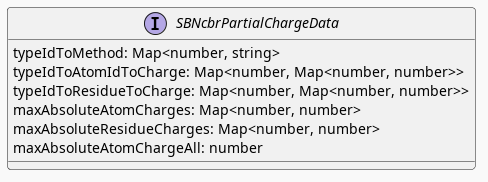
\includegraphics[width=\textwidth]{out/figures/uml/interface/custom model property interface.png}
  \end{center}
  \caption{Interface of the custom model property for storing partial atomic charges.}
  \label{fig:property_provider_interface}
\end{figure}


\begin{figure}[htbp]
  \caption{Interface of the custom model property for storing partial atomic charges.}
  \label{fig:custom_model_property}
  \definecolor{LightGray}{gray}{0.95}
  \begin{minted}[
  frame=lines,
  framesep=2mm,
  baselinestretch=1.2,
  bgcolor=LightGray,
  fontsize=\footnotesize,
  % linenos
  ]{Typescript}
    type TypeId = number;
    type IdToCharge = Map<number, number>;
    export interface SBNcbrPartialChargeData {
        typeIdToMethod: Map<TypeId, string>;
        typeIdToAtomIdToCharge: Map<TypeId, IdToCharge>;
        typeIdToResidueToCharge: Map<TypeId, IdToCharge>;
        maxAbsoluteAtomCharges: IdToCharge;
        maxAbsoluteResidueCharges: IdToCharge;
        maxAbsoluteAtomChargeAll: number;
        params: PartialChargesPropertyParams;
    }
  \end{minted}
\end{figure}

\subsection{Color theme provider}
\label{subsection:color_theme_provider}

TODO: mention the color parameters \\

This provider serves as the central component of the extension, with its primary function being to assign colors to atoms and residues based on their charges. It achieves this by using the ColorTheme API provided by Mol*. The ColorTheme API is a mechanism for assigning colors to structural elements of a molecule. These structural elements can be atoms, residues, bonds, and so on. The API is based on the concept of a ColorTheme object, which is a collection of color assignments for structural elements. The ColorTheme object is then used by the Mol* library to color the structural elements of the molecule.

For the purposes of this extension, it was necessary to color two structural elements - atoms and residues. For both of these structural elements the charges were retrieved from the provider described in the previous section \ref{subsection:charges_provider}, which provided charges for atoms and residues.

To establish the color for a given charge, two color interpolations are employed: one for negative charges and another for positive charges. Atoms with positive charges receive a color from a white-to-blue color interpolation, while atoms with negative charges are assigned a color from a white-to-red color interpolation. These color interpolations are highlighted in Figure \ref{}. 

\begin{figure}[htbp]
  \centering
  \subfigure[Ball and stick]{\label{fig:partial_charges_color_theme-bas}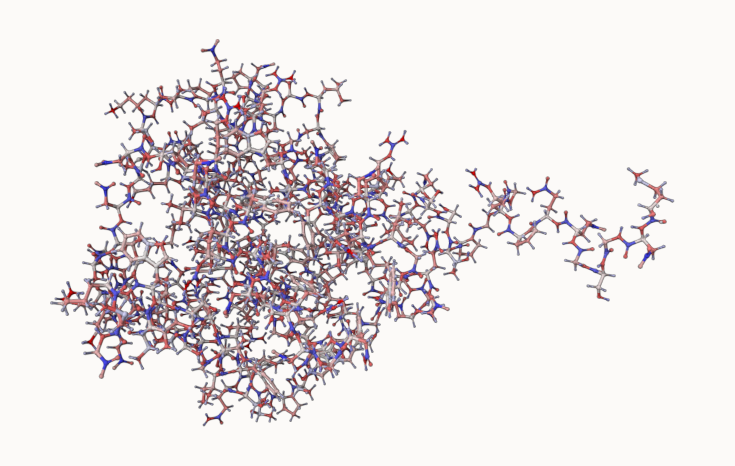
\includegraphics[width=0.45\textwidth]{figures/1F16-bas.png}}
  \subfigure[Surface]{\label{fig:partial_charges_color_theme-surface}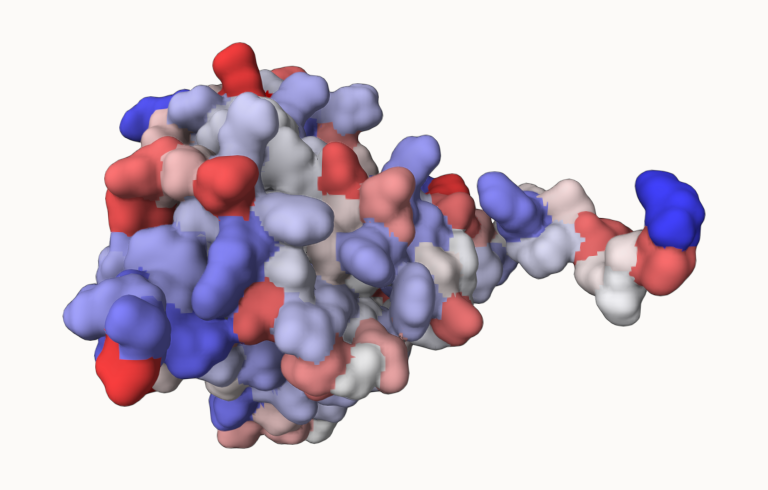
\includegraphics[width=0.45\textwidth]{figures/1F16-surface.png}}
  \subfigure[Cartoon]{\label{fig:partial_charges_color_theme-cartoon}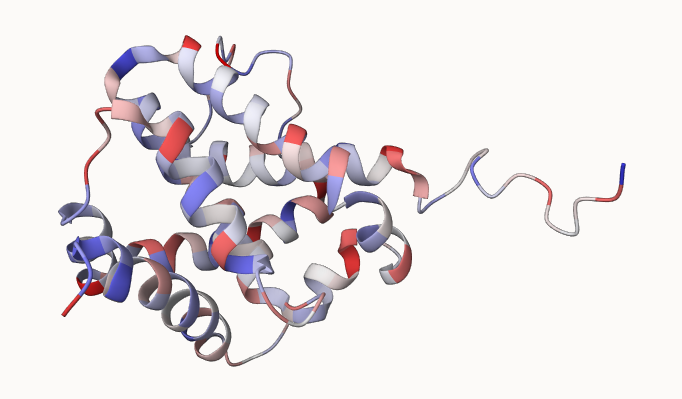
\includegraphics[width=0.45\textwidth]{figures/1F16-cartoon.png}}
  \caption{Partial charges color theme for different visualization types.}
  \label{fig:partial_charges_color_theme}
\end{figure}

\subsection{Label provider}
\label{subsection:label_provider}

Having colored the structural elements, it was also necessary to create a label provider, which would assign labels that describe the charge of the structural element. In order to determine which element is highlighted, Mol* uses the object Loci. A Loci object is utilized for general selections and highlights. Consequently, it is essential to first extract the location from the Loci object in order to obtain the atom ID. The charge is acquired from the property provider, and the label is an HTML string that conveys the charge of the atom or residue. An example of the label can be seen in in the right-hand corner in figure \ref{}.

\subsection{Controls}
\label{subsection:controls}

The controls are implemented automatically by the Mol* library based on the parameters of the providers. The user has access to controls of the charge set and the color theme. The charge set controls allow the user to select the charge set to display. The color theme controls allow the user to specify the following parameters:

\begin{itemize}
  \item \textbf{Charge Range}: Sets the range of the color interpolation
  \item \textbf{Use Range}: Toggles whether the range of the color interpolation is automatically calculated or manually specified.
  \item \textbf{Charge Type}: Selects whether to display the partial atomic charges or the partial residue charges.
\end{itemize}

The controls are depicted in Figure \ref{fig:controls-charge-set}.

\begin{figure}[htbp]
  \centering
  \subfigure[Charge set controls]{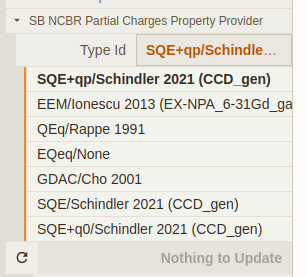
\includegraphics[width=0.45\textwidth]{figures/controls-charge-set.png}}
  \subfigure[Color theme controls]{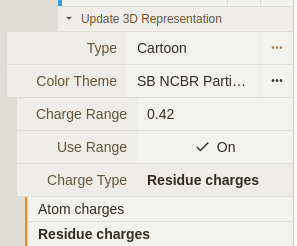
\includegraphics[width=0.45\textwidth]{figures/controls-color-theme.png}}
  \caption{Extension controls.}
  \label{fig:controls-charge-set}
\end{figure}

\section{Mol* viewer plugin}
\label{chapter:molstar_viewer_plugin}

In addition to the partial charges extension for the Mol* library, it was necessary to create a custom Mol* viewer plugin. By using a plugin, it is possible to create custom behavior for the Mol* viewer, which is not possible using the standard Mol* viewer.

The plugin is implemented as a Typescript class which contains a method for creating the plugin, loading structure files, and four properties that serve as an interface for the plugin. 

The color themes and visualization types are changed by iterating over the Mol* state tree and changing each representation node.

\chapter{Atomic Charge Calculator II}
\label{chapter:atomic_charge_calculator_ii}

Atomic Charge Calculator II (ACC2) is a web application for calculating partial atomic charges for structure files. The application is built using Flask for the backend and Javascript with Bootstrap for the frontend. The core of the ACC2 application is the ChargeFW2 program, which is used to calculate the partial atomic charges. For visualizing the calculation results, the application uses the Litemol software. \cite{racek2020acc2} However, since the Litemol software is no longer supported, it was necessary to replace it with its modern counterpart, Mol*.

This chapter describes the changes made to the ACC2 application. We first discuss the modifications to the ChargeFW2 program, then explain the changes made to the backend and frontend to support calculations of multiple charge sets, and lastly we describe the integration of the Mol* viewer into the ACC2 application.

\section{Extension of ChargeFW2}
\label{section:chargefw2_extension}

As discussed in \ref{subsection:chargfw2}, ChargeFW2 is a C++ program for computing partial atomic charges. The program supports the following input file formats: SDF, MOL2, PDB, and mmCIF, all of which are described in Section \ref{section:chemical_file_formats}. The program parses the necessary atom and bond data for each molecule in the input file and stores it in a \texttt{Molecule} object. These objects are then stored in a \texttt{MoleculeSet} object over which the program then iterates and calculates the partial atomic charges for each molecule.

The program outputs the charge results in multiple file formats. The following table \ref{table:chargefw2_output_formats} lists the output file formats generated by ChargeFW2 for the corresponding input file formats.

\begin{table}[htbp]
  \centering
  \begin{tabular}{|l|l|}
    \hline
    \textbf{Input format} & \textbf{Output formats} \\
    \hline
    SDF, MOL2 & TXT, MOL2 \\
    \hline
    PDB & TXT, PQR \\
    \hline
    mmCIF & TXT, PQR, mmCIF \\
    \hline
  \end{tabular}
  \caption{ChargeFW2 output file formats.}
  \label{table:chargefw2_output_formats}
\end{table}

As can be seen in Table \ref{table:chargefw2_output_formats}, ChargeFW2 already outputs a mmCIF file. However, the format of this mmCIF file stores the partial atomic charges in a custom \texttt{\_atom\_site.fw2\_charge} item, and therefore, it is not compatible with the Mol* viewer, which expects the partial atomic charges to be stored in the custom mmCIF categories described in Section \ref{section:custom_mmcif_categories}.

The following subsections describe in detail how ChargeFW2 was modified to produce the custom mmCIF file format for all the input files, regardless of the input file format.

\subsection*{mmCIF}

For mmCIF input files, the program simply appends the custom categories to the input file. To add the categories, the program uses the GEMMI library \cite{wojdyr2022gemmi} to parse the input mmCIF file into a \texttt{Block} object, which provides access to all mmCIF categories in the file. Before appending the charge categories, the program first removes alternative conformations from the \texttt{Block} object. This is necessary because the Mol* viewer does not support alternative conformations. The program then appends the custom charge categories to the \texttt{Block} object and writes the \texttt{Block} object to a new mmCIF file.

\subsection*{PDB}

The PDB input files are first converted to mmCIF format using the GEMMI library. To achieve this, the PDB file is first parsed into a \texttt{Structure} object, which is then converted into a \texttt{Block} object. After converting the PDB file to mmCIF, it was necessary to remove the \texttt{\_chem\_comp} category from the \texttt{Block} object. This category is generated by GEMMI by default, however, it is not necessary for the Mol* viewer and its presence causes the viewer to visualize the structure incorrectly. The program then proceeds in the same way as for the mmCIF input files.

\subsection*{SDF and MOL2}

Both SDF and MOL2 input files are converted to mmCIF format using the atom and bond data parsed from the input file. The program first creates an empty \texttt{Block} object, which it then populates with the \texttt{\_atom\_site} and \texttt{\_chem\_comp\_bond} categories. The program then proceeds in the same way as for the mmCIF input files.

\subsection*{Summary}

The ChargeFW2 was modified to produce a mmCIF file for each calculation, which is compatible with the Mol* viewer. The Table \ref{table:new_chargefw2_output_formats} lists the updated output file formats generated by ChargeFW2 for the corresponding input file formats.

\begin{table}[htbp]
  \centering
  \begin{tabular}{|l|l|}
    \hline
    \textbf{Input format} & \textbf{Output formats} \\
    \hline
    SDF, MOL2 & TXT, mmCIF, MOL2 \\
    \hline
    PDB, mmCIF & TXT, mmCIF, PQR \\
    \hline
  \end{tabular}
  \caption{Updated ChargeFW2 output file formats.}
  \label{table:new_chargefw2_output_formats}
\end{table}

\section{Multicharge support}
\label{section:multicharge_support}

The ACC2 application allows the user to select the method and parameters that will be used to calculate the partial atomic charges for the user's input file. Once the user confirms their selection, the application sends it to the backend, which runs the ChargeFW2 program with the chosen method and parameters. The application then displays the results of the calculation to the user. However, the application only supports one calculation per request and does not support the visualization of multiple charge sets. This limitation was previously caused by the Litemol viewer, which only supported one charge set per structure. However, since the Mol* viewer supports multiple charge sets, the ACC2 application was modified to support multiple charge sets as well.

The following subsections describe the necessary changes made to the ACC2 application to facilitate multiple calculations per one request and the visualization of multiple charge sets.

\subsection{Frontend changes}

As previously explained in section \ref{section:multicharge_support}, the ACC2 application used to limit the user to selecting only one combination of method and parameters. This limitation was resolved by introducing new controls to the calculation setup.

Figure \ref{fig:new_setup} shows the updated setup page for the ACC2 application. The page now contains a list of calculations, where each calculation represents a combination of method and parameters. The list is initially empty and the user can add a new calculation to the list by selecting the desired method and parameters from the drop-down menus and clicking the \textit{Add to calculation} button. The user can also remove any calculation from the list by clicking the cross button next to the calculation name. The list of calculations is then sent to the backend where it is used to generate the desired charge sets for the user's input file.

\begin{figure}[htbp]
  \begin{center}
    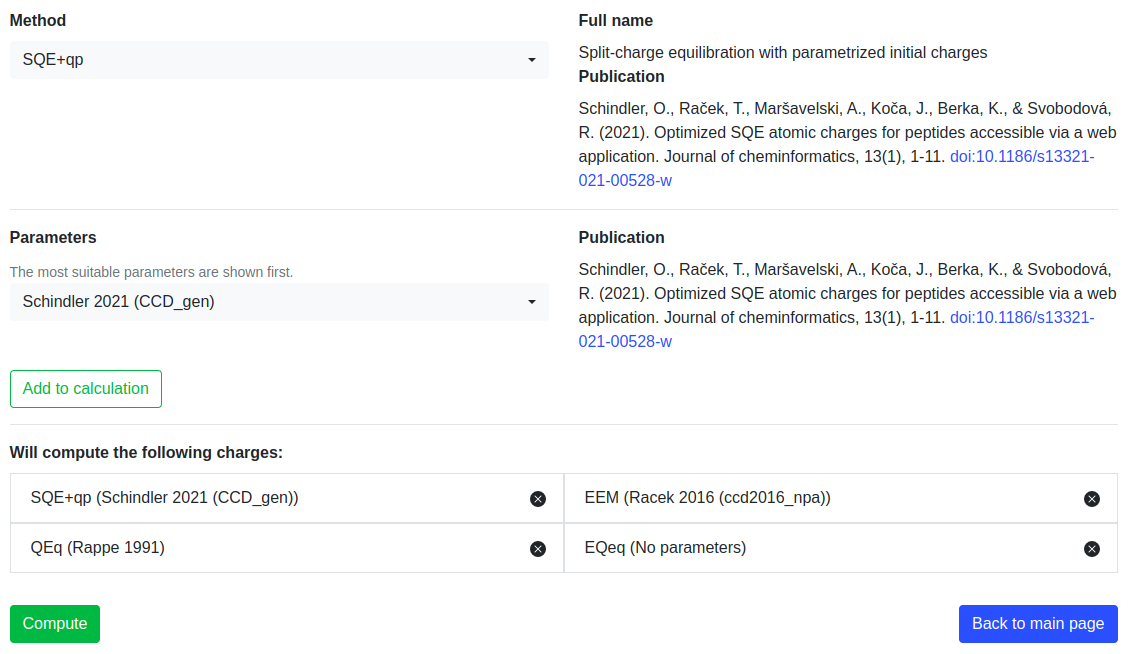
\includegraphics[width=\textwidth]{figures/new_setup.png}
  \end{center}
  \caption{Updated setup page for the ACC2 application.}
  \label{fig:new_setup}
\end{figure}

\subsection{Backend changes}

The Flask backend of the ACC2 application was modified to support multiple calculations per request. The backend now receives a list of calculations from the frontend, which it uses to generate the desired charge sets for the user's input file. It does this by running the ChargeFW2 program for each calculation in the list. For each calculation the ChargeFW2 generates the output file formats described in Table \ref{table:new_chargefw2_output_formats}. The backend then parses the charge values from the output TXT file and stores them in a dictionary, creating a mapping between the charge set name and the charge values.

After all the calculations have been completed, the dictionary is used to generate the mmCIF file. Firstly, the backend parses one of the output mmCIF files generated by ChargeFW2 into a \texttt{Block} object using the GEMMI library. The backend then iterates over dictionary and appends the charge values to the \texttt{Block} object under the custom charge categories. Lastly, the backend writes the \texttt{Block} object to a new mmCIF file, which is then sent to the frontend, where it is loaded into the Mol* viewer.

\section{Mol* viewer integration}
\label{section:viewer_integration}

Figure \ref{fig:result_page} shows the result page for the ACC2 application with the Mol* viewer. The Mol* viewer is integrated into the result page by initializing the custom viewer plugin, loading the mmCIF file generated by the backend, and configuring the viewer to visualize the charge values.

Additionally, the page allows the user to change the coloring and visualization of the structure. The structure can be visualized as a ball-and-stick model, as a surface model, or if applicable as a cartoon model. The user has also the option to choose the coloring. The structure can be colored by partial atomic charges or by the element symbol of each atom. The user can also set the maximum charge value that will be used for the coloring or reset the maximum charge value to the default value.

The user can download all the output files generated by the backend by clicking the \textit{Download charges} button. This button downloads a ZIP archive containing all the output files, which are organized into folders for each file format.

\begin{figure}[htbp]
  \begin{center}
    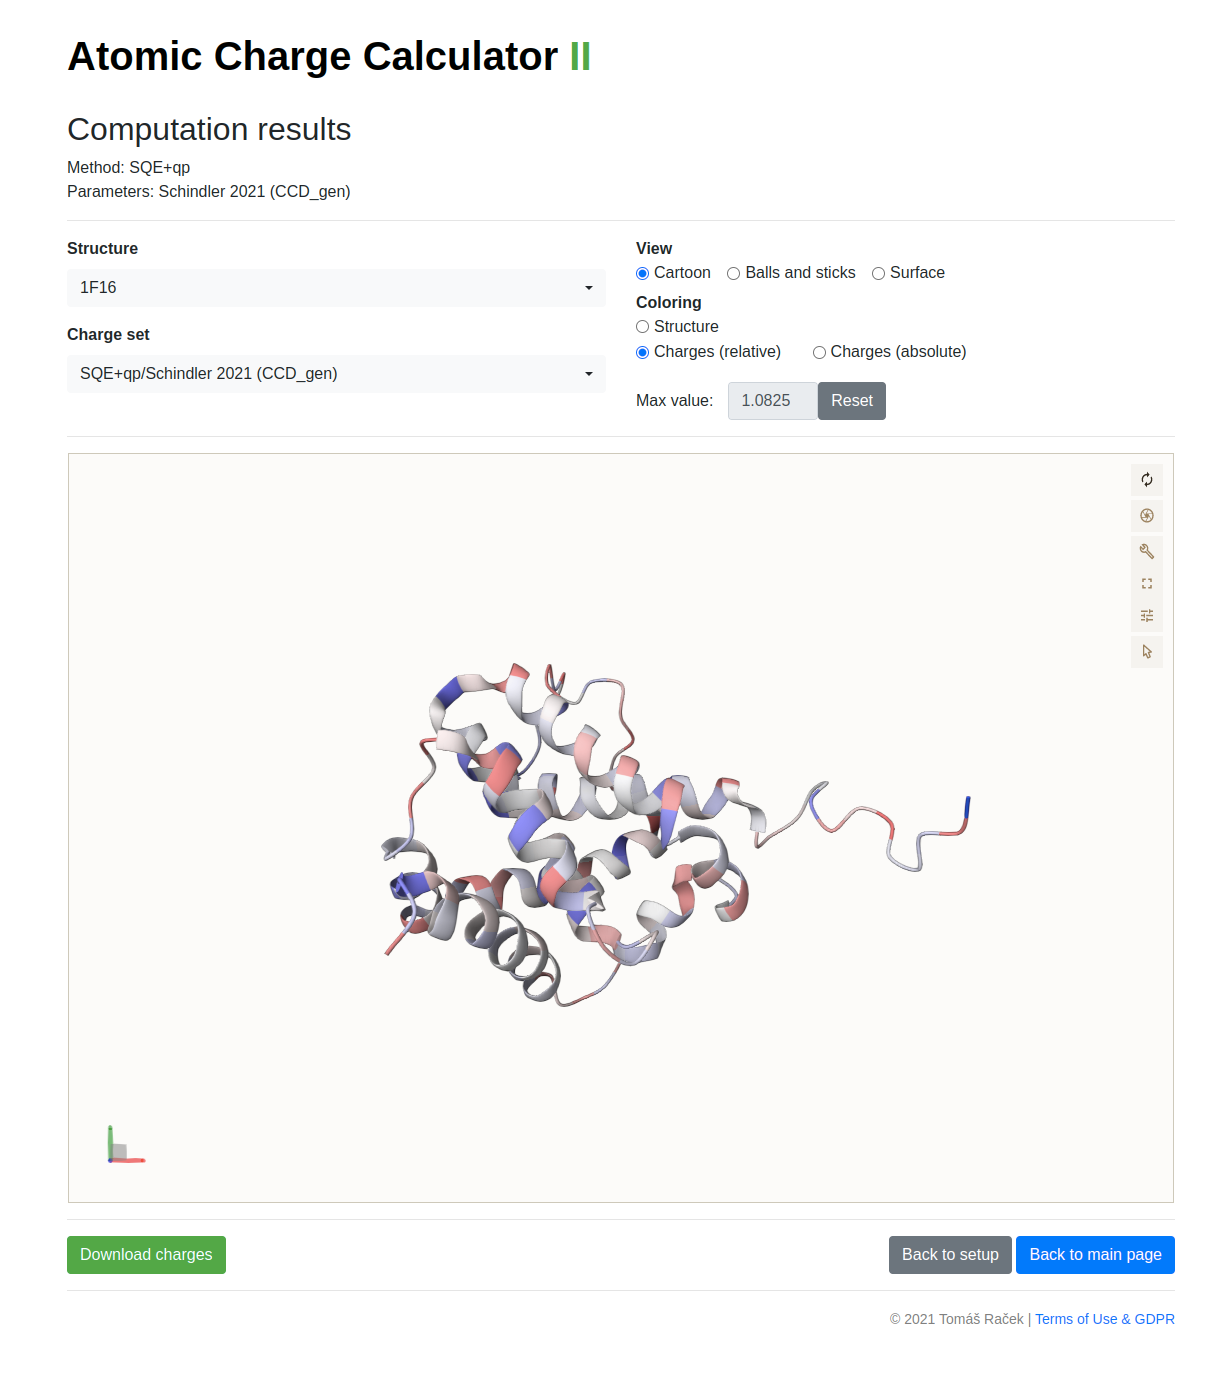
\includegraphics[width=\textwidth]{figures/results-full.png}
  \end{center}
  \caption{Result page for the ACC2 application with the Mol* viewer.}
  \label{fig:result_page}
\end{figure}

\chapter{AlphaCharges}

AlphaCharges (αCharges) is a web application for calculating partial atomic charges for structures from AlphaFoldDB, a database of protein structures predicted by AlphaFold2 \cite{jumper2021alphafold}. The AlphaCharges application protonates the protein structures (i.e. adds hydrogens) and calculates the partial atomic charges for the structures with the SQE+q0 empirical method \cite{schindler2021sqe}. \cite{schindler2023alphacharges}

During the development of the AlphaCharges application, the Mol* viewer was incorporated into the application to visualize the calculated partial atomic charges. The following sections describe the changes made to the Mol* viewer to support the AlphaCharges application and the integration of the Mol* viewer into the application.

\section{Integration of the the Mol* viewer}

\textbf{TODO}: explain the conversion of PDB into mmCIF and addition of ma\_qa mmCIF categories with confidence scores \\

The AlphaCharges application shares the architecture with the ACC2 application. The frontend is written in Javascript with the Bootstrap framework, the backend is written in Python and uses the Flask framework. This shared architecture allowed the integration of the Mol* viewer into the AlphaCharges application with minimal adjustments. As with the ACC2 application, the Mol* viewer is incorporated into the result page by initializing the plugin viewer, loading the mmCIF file generated by the backend, and mounting the controls for managing the viewer.

The creators of the AlphaCharge application requested the addition of two new features to the Mol* viewer. Firstly, the creators requested the addition of a new color theme for the coloring of the structure by the pLDDT confidence score. Secondly, the creators requested a focus control for the viewer, which would allow the user to focus (i.e. zoom in and center) on a specific atom in the structure. The following subsections describe the implementation of the new features.

% The controls for changing the coloring and visualization type of the structures function in the same way as in the ACC2 application. However, the AlphaCharges application requires an additional control for selecting the coloring by the pLDDT confidence score. Moreover, the AlphaCharges application does not support switching between multiple structures or switching between multiple charge sets. Therefore, the dropdown menus for selecting the structure and the charge set were ommited from the result page.

% The figure \ref{fig:alpha-charges-results} shows the result page for the AlphaCharges application. The additional control for changing the coloring of the structure by the pLDDT confidence score is highlighted in red.

\subsection{Coloring by pLDDT confidence score}

AlphaFold2 generates a confidence score for each residue in the predicted protein structures using a measure called pLDDT. The confidence score is a value ranging between 0 and 100, where higher values indicate higher confidence levels. \cite{varadi2021alphafold} The AlphaFoldDB includes the confidence scores along with the predicted protein structures in the mmCIF file format. These confidence scores are stored in the mmCIF file under the following categories:

\textbf{TODO}: the descriptions in the following list are taken from PDBx/mmCIF; how can i cite this? \\

\begin{itemize}
  \item \texttt{\_ma\_qa\_metric} - contains details of the metrics use to assess model quality.
  \item \texttt{\_ma\_qa\_metric\_local} - contains information about the local QA metrics calculated at the residue-level.
  \item \texttt{\_ma\_qa\_metric\_global} - contains information about the global QA metrics calculated at the model-level.
\end{itemize}

To support this feature, the Mol* viewer was extended to include a color theme provided by the Mol* library for visualizing the pLDDT confidence score. This pLDDT color theme uses a set of colors ranging from orange to blue, where orange indicates low confidence and blue indicates high confidence. The color theme is applied to the structure by mapping the pLDDT scores to the set of colors.

To incorporate this coloring in AlphaCharges, the custom Mol* viewer plugin was extended to include a function for switching to the pLDDT color theme. The AlphaCharges application then uses this function to add a new coloring control to the result page. This control is similar to the existing coloring controls, which allow the user to color the structure by the element symbol or by the partial atomic charges. The pLDDT coloring control is shown in Figure \ref{fig:alpha-charges-results}.

\begin{figure}[htbp]
  \begin{center}
    \includegraphics[width=\textwidth]{figures/alpha-charges-results.png}
  \end{center}
  \caption{Result page of the AlphaCharges application. The control for switching to the pLDDT color theme is highlighted in red.}
  \label{fig:alpha-charges-results}
\end{figure}

\subsection{Focus on problematic atoms}

The AlphaCharges application cannot calculate the partial atomic charges for all protein structures. Some structures can be incorrectly predicted by the AlphaFold2 algorithm or the application can fail to protonate the structure.
\cite{jumper2021alphafold} In such instances, the application automatically redirects the user to an error page, which displays the problematic structure and the error message.

We cover the implementation of the error page in more detail in the next section \ref{}. For the purpose of this section, it is sufficient to know that the error page contains an error message with the atoms that caused the error. The user has an option to click on the problematic atoms to focus on them in the structure. This feature needed to be implemented in the Mol* plugin viewer.

% The user has the option to hover over the problematic atoms to display an explanation for the probable cause of the error. Figure \ref{fig:wrong_structure_text} shows the explanation provided for the atom \textit{GLN 33 CD}.

\begin{figure}[htbp]
  \begin{center}
    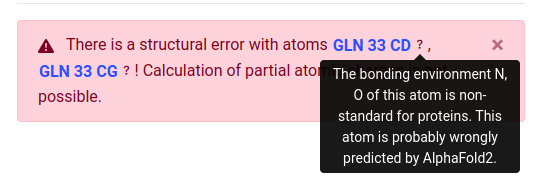
\includegraphics[width=\textwidth]{figures/wrong_structure_text.png}
  \end{center}
  \caption{Explanation for error of atom \textit{GLN 33 CD}.}
  \label{fig:wrong_structure_text}
\end{figure}

The Mol* library provides a function to focus on a specific structure selection. The selection can be created programmatically using the Mol* query language. The query language is built using the Molscript language \cite{kraulis1991molscript} and allows the user to select atoms based on their properties, such as their element symbol or their residue name.

To focus on the problematic atom \textit{GLN 33 CD}, displayed in Figure \ref{fig:wrong_structure_text}, the query language was used to first select the atom with the residue name \textit{GLN}, the residue number \textit{33}, and the atom name \textit{CD}. This combination of properties uniquely identifies the problematic atom in the structure. Then the selected atom was focused using the Mol* focus function. Figure \ref{fig:wrong_structure_focus} shows the Mol* viewer with the atom \textit{GLN 33 CD} focused.


\section{Problematic atoms webpage}

\textbf{TODO}: should this be merged into the previous section? \\ 

The backend sends a JSON object to the frontend containing problematic atoms and the explanations. Figure \ref{} shows the structure of the JSON schema. This JSON object is then used by the frontend to display the problematic atoms and their explanations.

The problematic atoms are added to the error message as a link. When the user clicks on the link, a event listener will be trigger, which will make the Mol* viewer focus on the problematic atom. Figure \ref{fig:wrong_structure_focus} shows the Mol* viewer with the atom \textit{GLN 33 CD} focused.

The user can also hover over a icon adjacent to the problematic atom to display the explanation for the probable cause of the error in a pop-up text. Figure \ref{fig:wrong_structure_text} shows the explanation provided for the atom \textit{GLN 33 CD}.

\begin{figure}[htbp]
  \begin{center}
    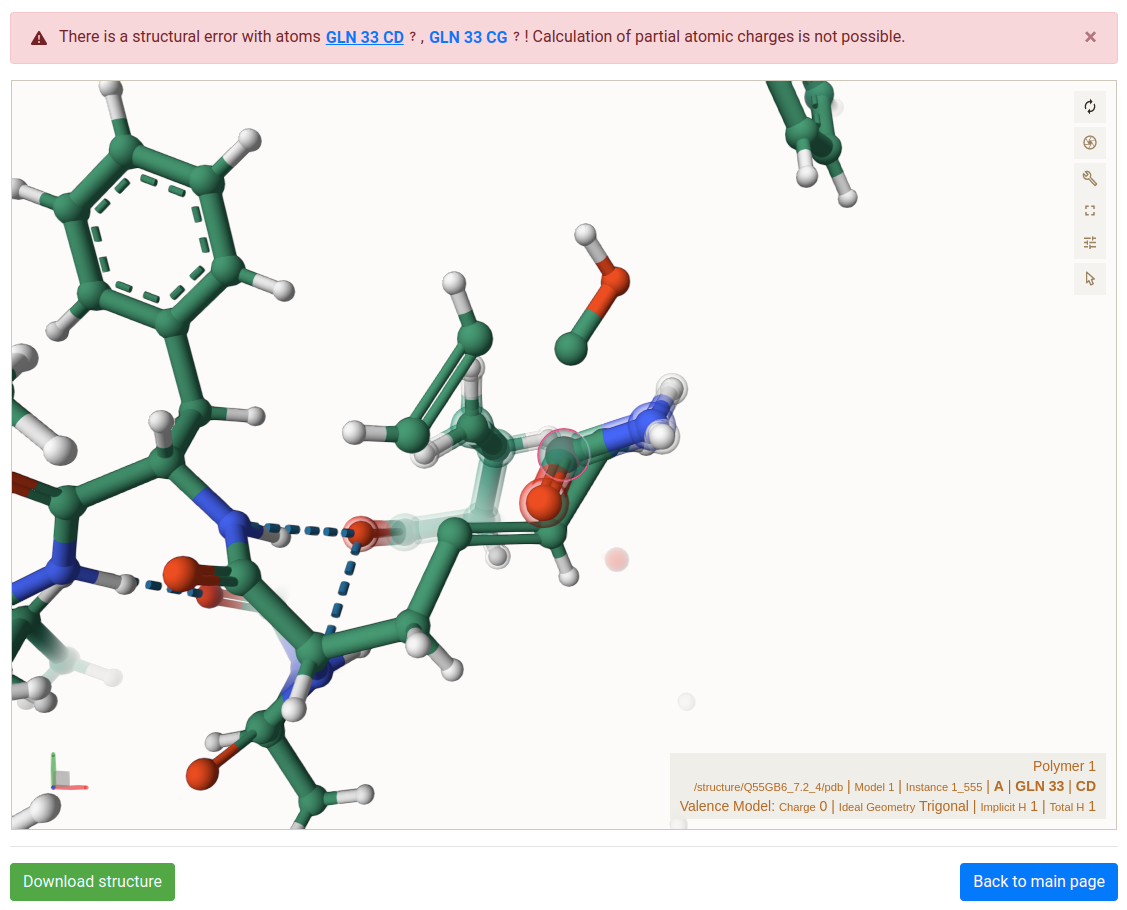
\includegraphics[width=\textwidth]{figures/wrong_structure_focus.png}
  \end{center}
  \caption{Focus on the atom GLN 33 CD, one of two problematic atoms in the structure with UniProt code Q55GB6.}
  \label{fig:wrong_structure_focus}
\end{figure}

\chapter*{Conclusion}
\markright{\textsc{Conclusion}}
\addcontentsline{toc}{chapter}{Conclusion}

\printbibliography[heading=bibintoc]

\end{document}
